\documentclass[electronic]{kthesis}

%%%%%%%%%%%%%%%%%
%%%% PACKAGES %%%
%%%%%%%%%%%%%%%%%
\usepackage[utf8x]{inputenc}
\usepackage[swedish,english]{babel}
\usepackage{enumerate}  % for capital latin numbers in the list of papers
\usepackage{caption}   % to align the table caption to the right/left
\usepackage{lscape}
\usepackage{hyperref}  %for references
\usepackage{amsmath,mathrsfs}
\usepackage{amssymb}  % assumes amsmath package installed
\usepackage{epstopdf}
\usepackage{subfig}
\usepackage{cite}
\usepackage{hyperref}
\usepackage{graphicx}
\usepackage{bm}	%Command \bm{make bold}
\usepackage{algorithm}
\usepackage{algpseudocode}
\usepackage{algpascal}
\usepackage{multicol}
\usepackage[x11names]{xcolor}
\usepackage{lipsum}

\usepackage{tikz}
\usetikzlibrary{tikzmark,calc,decorations.pathreplacing}
\newcommand{\Depth}{2}
\newcommand{\Height}{2}
\newcommand{\Width}{2}

\renewcommand{\labelitemi}{\textcolor{IndianRed3}{\bfseries\textbullet}}


%%%%%%%%%%%%%%%%%%%%%%%%%%%%%%%%%%%%%%%
%%%%%%%%% Document starts here %%%%%%%%
%%%%%%%%%%%%%%%%%%%%%%%%%%%%%%%%%%%%%%%
\begin{document}
	
	%%%%%%%%%%%%%%%%%%%%%%%%%%%%%%%%%%%%%%%%%%
	%%%%%% First and second pages %%%%%%%%%%%%
	%%%%%%%%%%%%%%%%%%%%%%%%%%%%%%%%%%%%%%%%%%
	\title{ Thesis Title }
	\subtitle{\textbf{sub-title}}
	\author{Marcus Klasson}
	\date{date}
	\thesistype{Doctoral Thesis}
	\imprint{Stockholm, Sweden, 2020}
	\examen{Teknologie doktorexamen i elektroteknik}
	\disputationsdatum{fredagen den 18 januari 2020 klockan 14.00}
	\disputationslokal{Sal F3, Lindstedtsvägen 26, Kungliga Tekniska H\"{o}gskolan, Stockholm}
	\publisher{Universitetsservice US AB}
	\address{KTH Royal Institute of Technology \\School of Electrical Engineering and Computer Science\\ Division of Fusion Plasma Physics \\ SE-10044 Stockholm\\ Sweden}
	\isbn{ISBN 100-}
	%\issn{ISSN XXX} % No longer used at KTH
	\trita{TRITA-EECS-AVL-2020:4}
	\kthlogo{KTHLogo}
	
	% Create title page using info above
	\maketitle
	
	\frontmatter % Pages i, ii, iii, iv, v etc.
	%%%%%%%%%%%%%%%%%%%%%%%%%%%%%%%%%%%
	%%%%%%%%%%% ABSTRACT %%%%%%%%%%%%%%
	%%%%%%%%%%%%%%%%%%%%%%%%%%%%%%%%%%%
	\begin{abstract}
		\noindent \lipsum[1]
		
	\end{abstract}
	
	\bigskip \bigskip \bigskip \bigskip \bigskip
	
	\setlength{\leftskip}{0.3 cm} \textbf {Keywords:} Lorem, Ipsum, Dolor, Sit, Amet
	
	%%%%%%%%%%%%%%%%%%%%%%%%%%%%%%%%%%%%%%%%
	%%%%%%%% SWEDISH ABSTRACT %%%%%%%%%%%%%%
	%%%%%%%%%%%%%%%%%%%%%%%%%%%%%%%%%%%%%%%%
	\newpage
	\selectlanguage{swedish}
	\begin{abstract}
		\noindent \lipsum[1]
	\end{abstract}
	\selectlanguage{english}
	
	%%%%%%%%%%%%%%%%%%%%%%%%%%%%%%%%%%%%%%%
	%%%%%%% List of papers %%%%%%%%%%%%%%%%
	%%%%%%%%%%%%%%%%%%%%%%%%%%%%%%%%%%%%%%%
	\chapter{List of Papers}
	
	\let\thefootnote\relax\footnote{Paper I and III are published under license in \textit{Journal of X}}
	\begin{enumerate}[I]
		\item \textbf{\textit{Title of paper}} \\
		\textbf{First author}, Second author \\
		\textit{Journal (year)}
	\end{enumerate}
	
	%%%%%%%%%%%%%%%%%%%%%%%% Papers NOT included in THESIS
	Other contributions by the author not included in the thesis.
	\begin{enumerate}[I]
		\setcounter{enumi}{1}
		\item \textbf{\textit{Title of paper}} \\
		\textbf{First author}, Second author \\
		\textit{Journal (year)}
	\end{enumerate}
	%%%%%%%%%%%%%%%%%%%%%%%%%%%%%%%%%%%%%%%
	%%%%%%%% ACKNOWLEDGMENT %%%%%%%%%%%%%%%
	%%%%%%%%%%%%%%%%%%%%%%%%%%%%%%%%%%%%%%%
	\chapter{Acknowledgement}
	\noindent \lipsum[1]
	
	%%%%%%%%%%%%%%%%%%%%%%%%%%%%%%%%
	%%%%%%%% ACRONYMS %%%%%%%%%%%%%%
	%%%%%%%%%%%%%%%%%%%%%%%%%%%%%%%%
	\chapter{Acronyms}
	List of commonly used acronyms: \\
	
	\begin{tabular}{llll}
		\textbf{AE}		&	Acronym examples \\
		\textbf{VAE}		&	Variational Autoencoder \\
		
	\end{tabular}
	
	%\input{Content/Dedication}\clearpage
	
	\mainmatter % Pages 1, 2, 3...
	%%%%%%%%%%%%%%%%%%%%%%%%%%%%%%%%%%%%%%
	%%%%%% TABLE OF CONTENTS %%%%%%%%%%%%%
	%%%%%%%%%%%%%%%%%%%%%%%%%%%%%%%%%%%%%%
	\tableofcontents
	
	%%%%%%%%%%%%%%%%%%%%%%%%%%%%%%%%%%%%%%%%%%%%%%%%%%%%%%
	%%%%%%%%%%%%% CHAPTER 1: INTRODUCTION %%%%%%%%%%%%%%%%
	%%%%%%%%%%%%%%%%%%%%%%%%%%%%%%%%%%%%%%%%%%%%%%%%%%%%%%
	\chapter{Energy needs - an introduction}
	\label{Intro}
	Here is an example for referencing figure \ref{EnergySources}. Example of citing \cite{BP2019} and \cite{Chen2016}.
	%%%%%%%%%%%%%% Figure: Energy sources
	\begin{figure}[h]
		\centering
		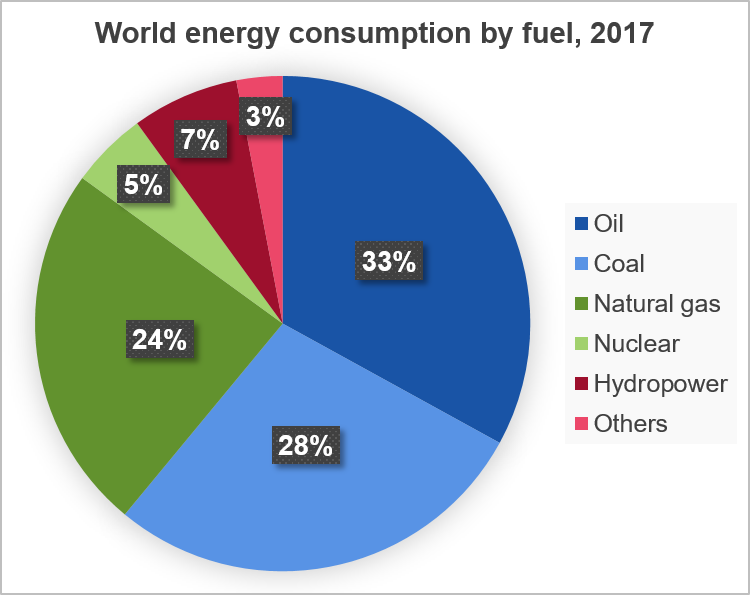
\includegraphics[scale=0.6]{Figs/Ch1_EnergySources.png}
		\caption{The world's energy consumption by fuel in 2017. }
		\label{EnergySources}
	\end{figure}
	
	%%%%%%%%%%%%%%%%%%%%%%%%%%%%%%%%%%%%%%%%
	\section{Section}
	Example of a table
	%%%%%%%%%%%%%%%%%%%%%%%%%%%%%%%% Table: Tokamaks
	\begin{table}[t!]
		\centering
		\caption{List of experimental tokamaks worldwide. Note: ITER is currently under construction and the first plasma is predicted for 2025-2028.}
		\begin{tabular}{ccccc}
			\hline
			\textbf{Name} & \textbf{Location} & \textbf{B-field} & \textbf{Major/minor radius}  \\
			\hline
			JET     & England      & 4.0 T & 3.0 m / 1.3 m \\
			ITER    & France       & 5.3 T & 6.2 m / 2.0 m \\
			AUG		& Germany      & 3.1 T & 1.7 m / 0.7 m \\
			WEST	& France	   & 3.7 T & 2.5 m / 0.5 m \\
			TCV     & Switzerland  & 1.5 T & 0.9 m / 0.3 m \\
			DIII-D  & USA          & 2.2 T & 1.7 m / 0.7 m \\
			TFTR 	& USA          & 6.0 T & 2.5 m / 0.9 m \\
			JT-60   & Japan        & 4.0 T & 3.4 m / 1.0 m \\
			K-STAR  & South Korea  & 3.5 T & 1.8 m / 0.5 m \\
			EAST    & China        & 3.5 T & 1.9 m / 0.5 m \\
			\hline
		\end{tabular}
		\label{TokamakTable}
	\end{table}
	
	
	\chapter{Chapter 2}
	\label{Ch2label}
	\noindent \lipsum[1]
	
	%%%%%%%%%%%%%%%%%%%%%%%%%%%%%%%%%%%%%%%%%%%%%%%%%%%%%%%%%%%%%%%%%%%%%%%%
	%%%%%%%%%%%%%%%%%%%%%%%%%%%%%%%%%%%%%%%%%%%%%%%%%%%%%%%%%%%%%%%%%%%%%%%%
	%%%%%%%%%%%%%%% CHAPTER 6: Summary of the publications %%%%%%%%%%%%%%%%%
	%%%%%%%%%%%%%%%%%%%%%%%%%%%%%%%%%%%%%%%%%%%%%%%%%%%%%%%%%%%%%%%%%%%%%%%%
	%%%%%%%%%%%%%%%%%%%%%%%%%%%%%%%%%%%%%%%%%%%%%%%%%%%%%%%%%%%%%%%%%%%%%%%%
	\chapter{Summary of the included papers}
	\label{Summary}
	\noindent \lipsum[1]
	
	%%%%%%%%%%%%%%%%%%%%%%%%%%%%%%%
	\section{Paper I - ...}
	
	%%%%%%%%%%%%%%%%%%%%%%%%%%%%%%%%%%%%%%%%%%%%%%%%%%%%%%%%%
	%%%%%%%%%%%%%%%%%%%%%%%%%%%%%%%%%%%%%%%%%%%%%%%%%%%%%%%%%
	%%%%%%%%%%%% CHAPTER 7: Conclusions %%%%%%%%%%%%%%%%%%%%%
	%%%%%%%%%%%%%%%%%%%%%%%%%%%%%%%%%%%%%%%%%%%%%%%%%%%%%%%%%
	%%%%%%%%%%%%%%%%%%%%%%%%%%%%%%%%%%%%%%%%%%%%%%%%%%%%%%%%%
	\chapter{Discussion and conclusions}
	\label{Conclusions}
	\noindent \lipsum[1]
	%%%%%%%%%%%%%%%%%%%%%%%%%%%%%%%
	
	%%%%%%%%%%%%%%%%%%%%%%%%%%%%%%%%%%%%%%%%%%%%%%%
	\section{Conclusions}
	\noindent \lipsum[1]
	
	%%%%%%%%%%%%%%%%%%%%%%%%%%%%%%%%%%%%%%%%%%%%%%%%%%%%%%%%%
	%%%%%%%%%%%%%%%%%%%%%%%%%%%%%%%%%%%%%%%%%%%%%%%%%%%%%%%%%
	%%%%%%%%%%%% CHAPTER 8: Personal reflections %%%%%%%%%%%%
	%%%%%%%%%%%%%%%%%%%%%%%%%%%%%%%%%%%%%%%%%%%%%%%%%%%%%%%%%
	%%%%%%%%%%%%%%%%%%%%%%%%%%%%%%%%%%%%%%%%%%%%%%%%%%%%%%%%%
	\chapter{Personal reflections}
	\label{PersonalReflections}
	\noindent \lipsum[1]
	
	%------------------------------------------------
	% CREATING THE BIBLIOGRAPHY
	%------------------------------------------------
	\bibliographystyle{ieeetr}
	\renewcommand{\bibname}{References}% changes default name Bibliography to References
	\bibliography{Refs} % References file
	
	%--------------------------------------------------
	
\end{document}
\endinput
%%
%% End of file `kth-demo.tex'.
